\section{Review}

\subsection{Area of Interest}
Area of Interest in this study is Balochistan.It is area wise largest province of Pakistan.
The extent is from $60.86989^o$ to $70.265642^o$ on East side and from $24.877092^o$ to $3262977^o$ to North side.
It consists of 37 districts, which are as show in figure \ref{fig:distInfo} and details are in table \ref{table:distInfo},
\begin{figure}[H]
    \centering
    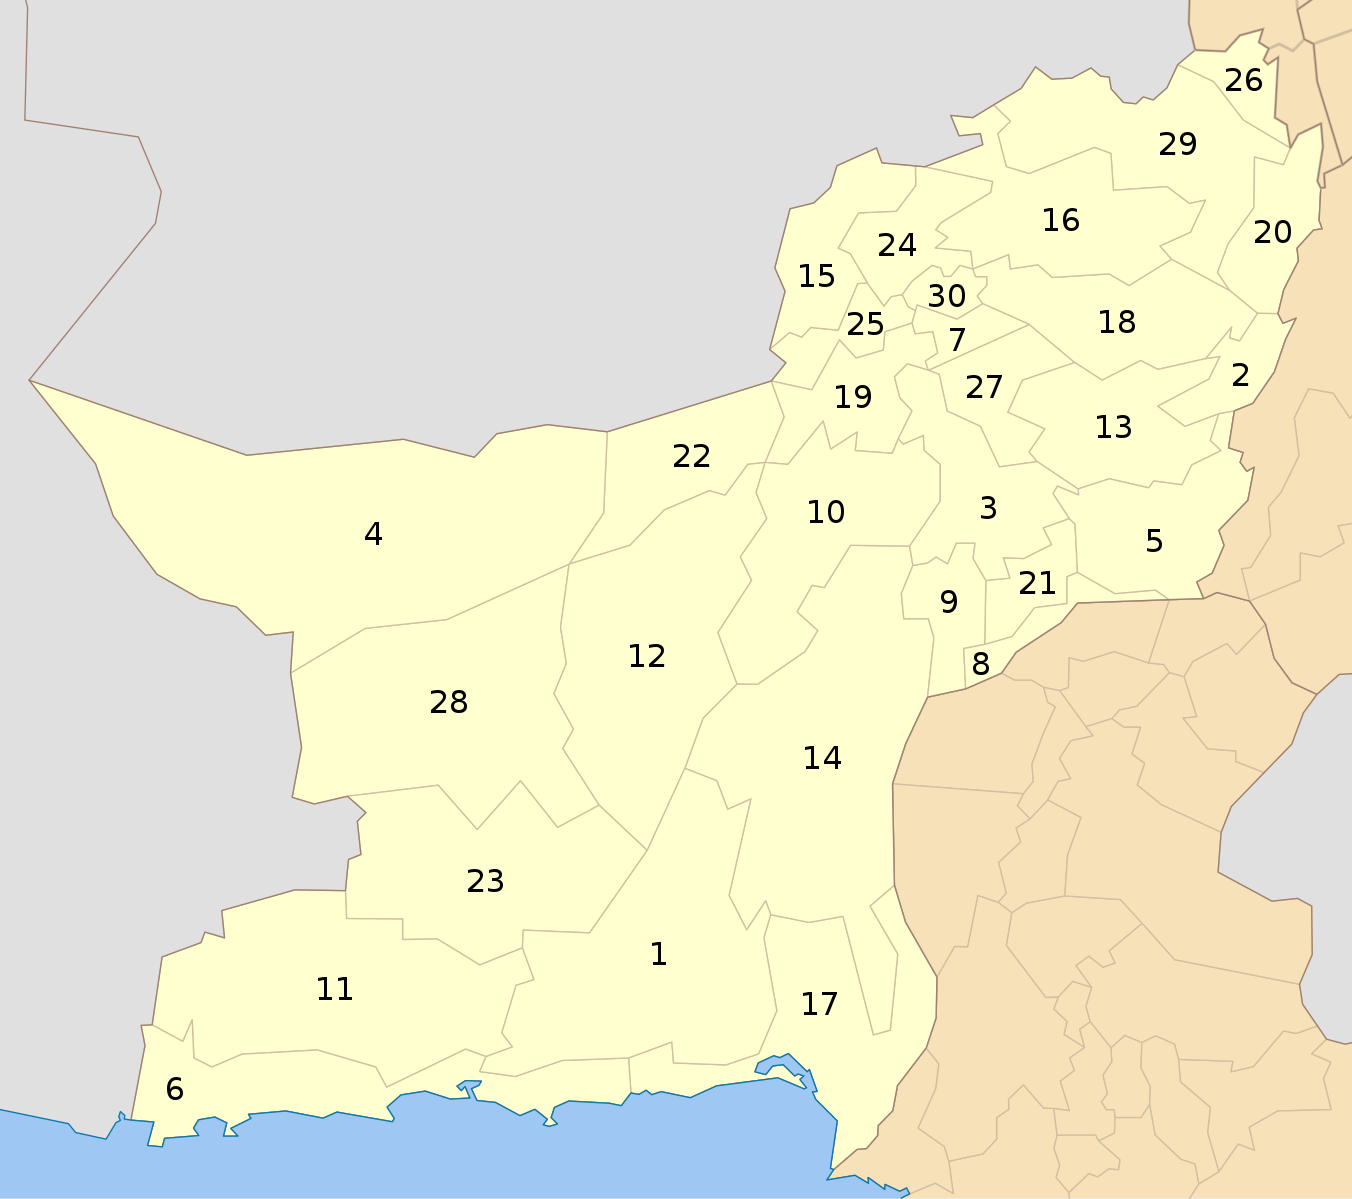
\includegraphics[width=0.6\textwidth]{images/Balochistan_Districts}
    \caption{District Information}\label{fig:distInfo}
\end{figure}
\begin{longtable}[H]{|p{0.05\linewidth} | p{0.2\linewidth} | p{0.2\linewidth} | p{0.1\linewidth} | p{0.1\linewidth} | p{0.1\linewidth}|}
    \hline
    Sr. No. & District       & Area (km2)                       & Population (1998) & Population (2017) & Density (pop/km2) \\
    \hline
    1       & Awaran         & 29510                            & 118173            & 121821            & 4                 \\
    2       & Barkhan        & 3514                             & 103545            & 171025            & 49                \\
    3       & Kachhi         & 5682                             & 255480            & 309932            & 55                \\
    4       & Chagai         & 44748                            & 104534            & 226517            & 5                 \\
    5       & Chaman         & 1341                             & 151854            & 434561            & 324               \\
    6       & Dera Bugti     & 10160                            & 181310            & 313110            & 31                \\
    7       & Duki           & 4233                             & 115976            & 152977            & 36                \\
    8       & Gwadar         & 12637                            & 185498            & 262253            & 21                \\
    9       & Harnai         & 2492                             & 76652             & 97052             & 39                \\
    10      & Hub            & 6716                             & 163194            & 339640            & 51                \\
    11      & Jafarabad      & 1643                             & 291290            & 513972            & 313               \\
    12      & Jhal Magsi     & 3615                             & 109941            & 148900            & 41                \\
    13      & Kalat          & 7654                             & 144433            & 211201            & 28                \\
    14      & Kech           & 22539                            & 413204            & 907182            & 40                \\
    15      & Kharan         & 14958                            & 96900             & 162766            & 11                \\
    16      & Kohlu          & 7610                             & 99846             & 213933            & 28                \\
    17      & Khuzdar        & 35380                            & 417466            & 798896            & 23                \\
    18      & Lasbela        & 8437                             & 149501            & 236631            & 28                \\
    19      & Loralai        & 3785                             & 134171            & 244446            & 65                \\
    20      & Mastung        & 3308                             & 150039            & 265676            & 80                \\
    21      & Musakhel       & 5728                             & 134056            & 167243            & 29                \\
    22      & Nasirabad      & 3387                             & 245894            & 487847            & 144               \\
    23      & Nushki         & 5797                             & 98030             & 178947            & 31                \\
    24      & Qila Abdullah  & 3553                             & 208870            & 323793            & 91                \\
    25      & Qila Saifullah & 6831                             & 193553            & 342932            & 50                \\
    26      & Panjgur        & 16891                            & 234051            & 315353            & 19                \\
    27      & Pishin         & 6218                             & 376728            & 736903            & 119               \\
    28      & Quetta         & 3447                             & 774547            & 2269473           & 658               \\
    29      & Sherani        & 4310                             & 81684             & 152952            & 35                \\
    30      & Sibi           & 7121                             & 136322            & 179751            & 25                \\
    31      & Sohbatpur      & 802                              & 141527            & 200426            & 250               \\
    32      & Surab          & 762                              & 93401             & 200857            & 264               \\
    33      & Washuk         & 33093                            & 110009            & 175712            & 5                 \\
    34      & Zhob           & 15987                            & 193458            & 310354            & 19                \\
    35      & Ziarat         & 3301                             & 80748             & 160095            & 48                \\
    36      & Karezat        & N/A (Part of Pashin district)    &                   &                   &                   \\
    37      & Usta Mohammad  & N/A (part of Jafarabad district) &                   &                   &                   \\
    \hline
    \caption{District Information}
    \label{table:distInfo}
\end{longtable}

\subsection{Basin Information}
The study area consist of 18 basins, which are as show in figure \ref{fig:basinInfo} and details are in table \ref{table:basinInfo}

\begin{figure}[H]
    \centering
    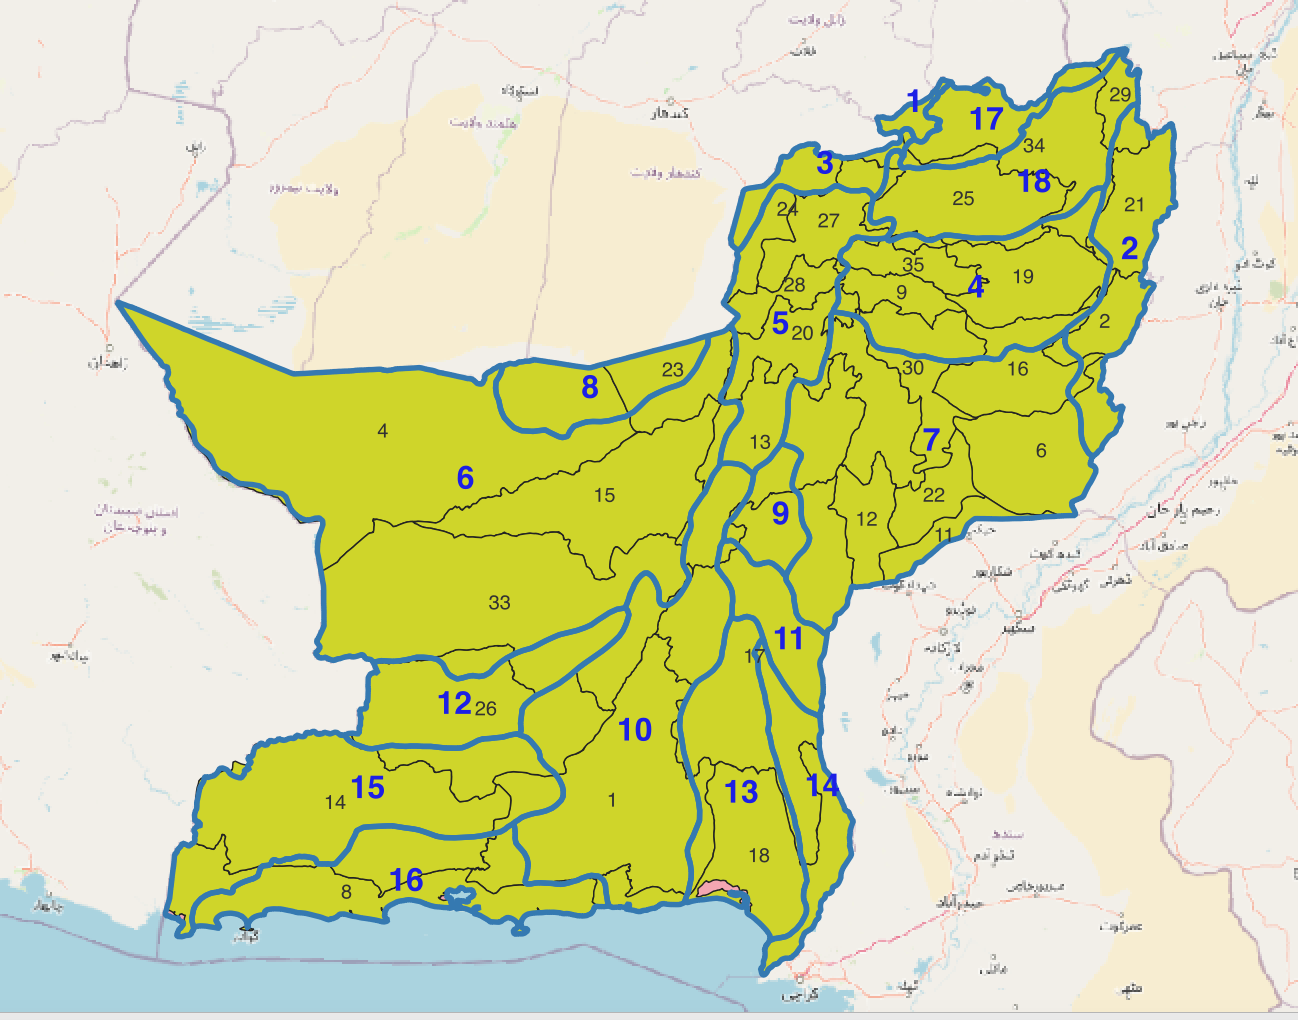
\includegraphics[width=0.6\textwidth]{images/bol_basins.png}
    \caption{Basin Map}\label{fig:basinInfo}
\end{figure}

\begin{longtable}[H]{| r l r |}
    \hline
    Basin Id & Name                   & Area      \\
    \hline
    1        & KAND RIVER BASIN       & 1117.406  \\
    2        & KAHA RIVER BASIN       & 12000.864 \\
    3        & KADNAI RIVER BASIN     & 4282.876  \\
    4        & NARI RIVER BASIN       & 21708.743 \\
    5        & PISHIN LORA BASIN      & 18152.095 \\
    6        & HAMUN-E-MASHKHEL BASIN & 85204.746 \\
    7        & KACHHI PLAIN BASIN     & 43575.396 \\
    8        & HAMUN-E-LORA BASIN     & 8281.098  \\
    9        & MULA RIVER BASIN       & 4670.923  \\
    10       & HINGOL RIVER BASIN     & 35548.887 \\
    11       & GAJ RIVER BASIN        & 6000.184  \\
    12       & RAKHSHAN RIVER BASIN   & 12322.828 \\
    13       & PORALI RIVER BASIN     & 18389.847 \\
    14       & HAB RIVER BASIN        & 8532.902  \\
    15       & DASHT RIVER BASIN      & 27644.378 \\
    16       & GWADAR-ORMARA BASIN    & 16975.713 \\
    17       & KUNDAR RIVER BASIN     & 6233.997  \\
    18       & ZHOB RIVER BASIN       & 16447.431 \\
    \hline
    \caption{Basins Information}
    \label{table:basinInfo}
\end{longtable}

Out of these 18 district four has been selected, i.e.,  Nari River Basin, Pishin Lora Basin, Hingol River Basin, and Hamon-e-Mashkhel Basin.
These basin are shown as shaded area in figure \ref{fig:selBasins} and their corresponding district are shown in table \ref{table:basin-dist}

\begin{figure}[H]
    \centering
    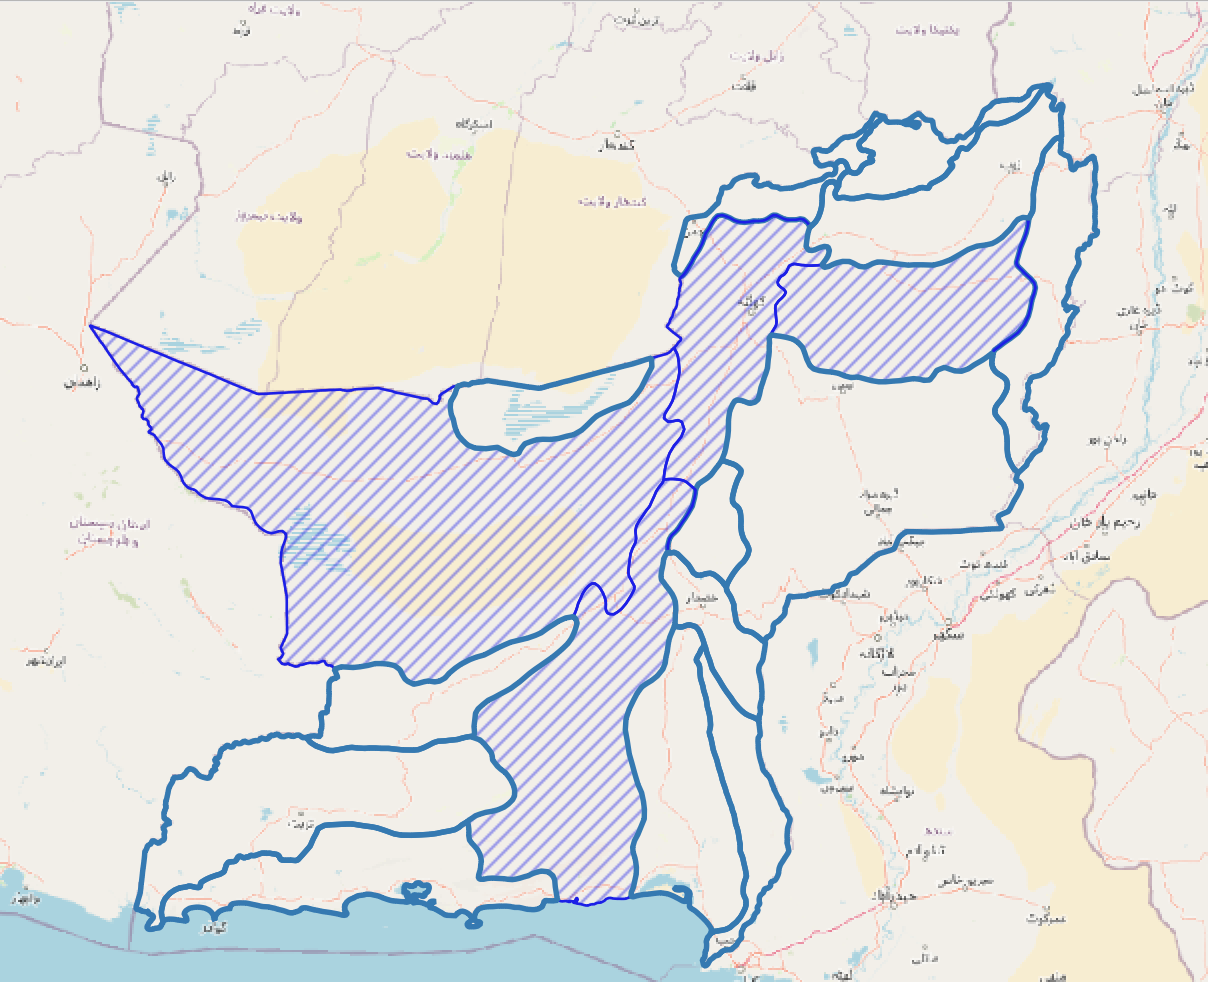
\includegraphics[width=0.6\textwidth]{images/SelectedBasins.png}
    \caption{Selected Basins}\label{fig:selBasins}
\end{figure}

\begin{longtable}[H]{| l | l | r |}
    \hline
    Basin                  & DISTRICT        & District\_tbl\_id \\
    \hline
    Hamun-e-Mashkhel Basin & Chagai          & 4.0               \\
    & Kalat           & 13.0              \\
    & Kharan          & 15.0              \\
    & Khuzdar         & 17.0              \\
    & Mastung         & 20.0              \\
    & Nushki          & 23.0              \\
    & Panjgur         & 26.0              \\
    & Quetta          & 28.0              \\
    & Washuk          & 33.0              \\
    \hline
    Hingol River Basin     & Awaran          & 1.0               \\
    & Gwadar          & 8.0               \\
    & Kalat           & 13.0              \\
    & Kharan          & 15.0              \\
    & Khuzdar         & 17.0              \\
    & Lasbela         & 18.0              \\
    & Panjgur         & 26.0              \\
    & Washuk          & 33.0              \\
    \hline
    Nari River Basin       & Barkhan         & 2.0               \\
    & Bolan           &                   \\
    & Harnai          & 9.0               \\
    & Kohlu           & 16.0              \\
    & Loralai         & 19.0              \\
    & Mastung         & 20.0              \\
    & Musakhel        & 21.0              \\
    & Pishin          & 27.0              \\
    & Qilla Saifullah & 25.0              \\
    & Quetta          & 28.0              \\
    & Sibi            & 30.0              \\
    & Zhob            & 34.0              \\
    & Ziarat          & 35.0              \\
    \hline
    Pishin Lora Basin      & Bolan           &                   \\
    & Harnai          & 9.0               \\
    & Kalat           & 13.0              \\
    & Mastung         & 20.0              \\
    & Nushki          & 23.0              \\
    & Pishin          & 27.0              \\
    & Qilla Abdullah  & 24.0              \\
    & Qilla Saifullah & 25.0              \\
    & Quetta          & 28.0              \\
    & Ziarat          & 35.0              \\
    \hline
    \caption{Basin Districts}
    \label{table:basin-dist}
\end{longtable}

\subsection{Methodology for Selection of River Basins}
A Spatial Multi-criteria analysis is conducted by Food and Agriculture Organization Pakistan(FAOPk) for the revival of water resources in Pakistan. The analysis is conducted at three level, i.e., River Basin level, District level, and Union Council level as shown in figure \ref{fig:MCARiver}.

\begin{figure}[H]
    \centering
    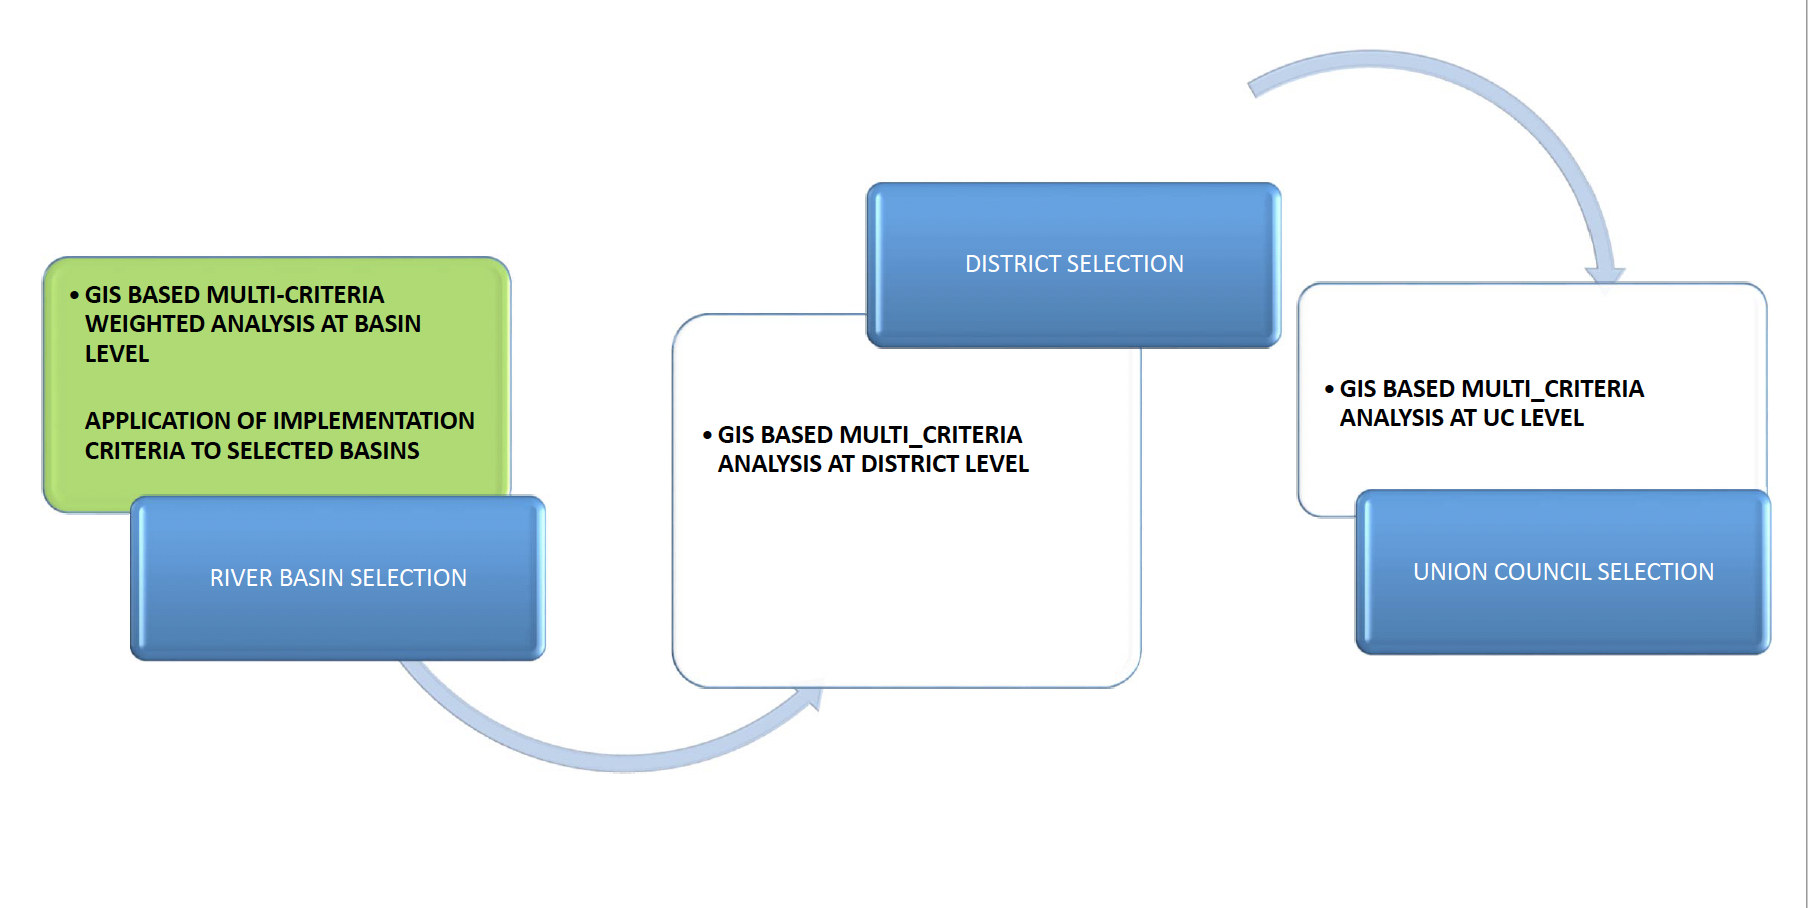
\includegraphics[width=0.6\textwidth]{images/MCARiver.png}
    \caption{Multi-Criteria Analysis Approach}\label{fig:MCARiver}
\end{figure}

At River basin level 5 criteria are utilized dividing into medium and high priority with 15\% and 20\% weightage respectively. The criteria are shown in table \ref{table:RiverBasinCriteria} and indicator used for these criteria are in table \ref{table:RiverBasinIndicator}

\begin{longtable}[H]{| l | l | l |}
    \hline
    Criteria                                           & Priority & Weigtage \\
    \hline
    Potential for Rainfed/Flood Plan Cropping          & Medium   & 0.15     \\
    Potential for Surface Water Harvesting             & Medium   & 0.15     \\
    Socio-Ecnomic Indicators                           & Medium   & 0.15     \\
    Potential for Water Conservartion                  & High     & 0.2      \\
    Potenttial for Enhancing Rangeland Production a... & High     & 0.2      \\
    \hline

    \caption{Criteria for River Basin Selection}
    \label{table:RiverBasinCriteria}
\end{longtable}

\begin{longtable}{| p{0.25\linewidth} | p{0.25\linewidth} | p{0.1\linewidth} | p{0.1\linewidth} | p{0.2\linewidth} |  }
    \hline
    Criteria                                        & Indicator Map                  & Unit             & Weightage & Source                                             \\
    \hline
    Potential for Water Conservation and Harvesting & Ground Water Depletion Index   &                  & 20.0 & Department of Irrigation, Government of Balochi... \\
    & Surplus Surface Water (MAF)    & BCM              & 15.0      & Department of Irrigation, Government of Balochi... \\
    \hline
    Potential for Livestock based Interventions     & Livestock Density              & Animal/250 sq.km & 20.0 & FAO Geonetwork \\
    \hline
    Potnetial for Enhancing Rangeland Production    & Area Under Rangeland           & Sq. km           & 15.0      & FAO, SUPARCO                                       \\
    \hline
    Potention for Rainfed Cropping                  & Area Under Rainfed / Floodplan & Sq. km           & 15.0      & FAO, SUPARCO                                       \\
    \hline
    Socio-Economic                                  & Food Inscurities               & \% of household  & 15.0      & UNDP, Ministry of Planning                         \\
    & Poverty Index                  &                  & -         & National Nutrition Survey                          \\
    & Population Density             &                  & -         & Census, 2017                                       \\
    \hline
    \caption {Indicator Maps for MCA of River Basin}
    \label{table:RiverBasinIndicator}
\end{longtable}

Based on these analysis 6 basins are shortlisted, i.e.,
\begin{itemize}
    \item Kacchi
    \item Nari
    \item Kaha
    \item Pishin
    \item Hamun‐e‐Mashkhel
    \item Hingol
\end{itemize}

\subsection{Methodology for Selection of Watershed}

For selection of watersheds a basin level River Basin Technical Working Groups have already been proposed. Approximately 8 watersheds in each basin will be finally selected based on a multicriteria decision analysis including step 1. Desk review and step 2. Rapid assessment in the watersheds to assess suitability. The selection of watersheds process initially begins in 2 rivers basins Pishin and Nari. Selection of watersheds will be tasked through the RB-TWG, in September, 2022.

To make a reference in June 2022 the selection process of the following 4 river basins have been completed through an established Multicriteria Decision Analysis (MCDA). The selected, yet to be notified, river basins include:
\begin{itemize}
    \item Pishin Lora Basin
    \item Nari River Basin
    \item Hamun e Maskel
    \item Hingol River Basin
\end{itemize}

Selection Criteria of each watershed will include a two steps approach.

\subsubsection{Step 1 Desk review of GIS MCDA by the River Basin Technical Working Group RB-TWG. }

This will be based on information extracted from ranking of watersheds derived through GIS based Multicriteria analysis for prequalification of high candidate watersheds where field assessment can proceeds. The results of GIS based MCDA for watersheds will be presented to the River Basin Technical Working Group for building for feedback and developing consensus. The GIS based MCDA considers Relevance to the RBWRP defined Result Areas as principal criterion summarized in the table below.

\begin{longtable}{| p{0.35\linewidth} | p{0.35\linewidth} | p{0.07\linewidth} | p{0.07\linewidth} | }
    \hline
    CRITERIA                                           & INDICATOR (watershed level)                        & WEIGHT & INF\\
    \hline
    Potential for Ground Water Recharge                & Average annual Rainfall (as an indicator of Wat... & 0.60 & 75\% weightage \\
    -                                                  & Area under Rangelands (sq.km)                      & 0.20                & -                             \\
    -                                                  & Area under Wetlands (sq.km)                        & 0.20                & -                             \\
    -                                                  & Total                                              & 1.00                & -                             \\
    Potential for Surface Water harvesting             & Average annual rainfall for 20 years (mm) & 0.70 & -\\
    -                                                  & Run-off potential based on soil texture            & 0.20                & -                             \\
    -                                                  & Population density                                 & 0.10                & -                             \\
    -                                                  & Total                                              & 1.00                & -                             \\
    Potential For Livestock Based Interventions        & Livestock Density                                  & 0.40                & -                             \\
    -                                                  & Area under rangelands (sq.km)                      & 0.60                & -                             \\
  \hline
    -                                                  & Total                                              & 1.00                & -                             \\
    \hline
    Potential for development of value chains for l... & To be done in Desk review and Rapid Assessment ... & 0.34 & 25\% Weightage \\
    Potential for command area development             & To be done in Desk review and Rapid Assessment ... & 0.33 & -\\
    Presence of community based Institutions with ...  & To be done in Desk review and Rapid Assessment ... & 0.33 & -\\
\hline
  &                                              Total &                 1.00 &                           -\\
\hline
\end{longtable}

\subsubsection{Step 2 Field level assessment in the prequalified watersheds}
Step 2 of the selection criteria is the Ground truthing by conducting field level assessment in the prequalified watersheds by RB-TWG consisting of NRM experts (from FAO and Landel Mills) with line department government field staff. A field assessment methodology will be developed well before the rapid assessment.
Based on above criteria Step 1 and Step 2 Recommendations for high candidate watershed will be formulated by the RB-TWG. Accordingly IWRM plans will be prepared based on the findings of GIS based decision analysis and ground truthing by rapid assessment in the field.
\b{Exclusion criteria for disqualification of include one or more of the following: }
\begin{enumerate}
	\item Areas with relatively low productivity potential for livestock and cropping in comparison to other areas that is % area falling under rugged and rough terrain
	\item Desert and hyper arid areas, (Annual Average Rainfall below 100 mm).
	\item Areas with High Security Risk
	
\end{enumerate}